\documentclass{article} % For LaTeX2e
\usepackage{nips14submit_e,times}
\usepackage{amsmath}
\usepackage{amsthm}
\usepackage{amssymb}
\usepackage{mathtools}
\usepackage{hyperref}
\usepackage{url}
\usepackage{algorithm}
\usepackage[noend]{algpseudocode}
%\documentstyle[nips14submit_09,times,art10]{article} % For LaTeX 2.09

\usepackage{mathrsfs}
\usepackage{graphicx}
\usepackage{caption}
\usepackage{subcaption}

\def\eQb#1\eQe{\begin{eqnarray*}#1\end{eqnarray*}}
\def\eQnb#1\eQne{\begin{eqnarray}#1\end{eqnarray}}
\providecommand{\e}[1]{\ensuremath{\times 10^{#1}}}
\providecommand{\pb}[0]{\pagebreak}


\def\Qb#1\Qe{\begin{question}#1\end{question}}
\def\Sb#1\Se{\begin{solution}#1\end{solution}}

\newenvironment{claim}[1]{\par\noindent\underline{Claim:}\space#1}{}
\newtheoremstyle{quest}{\topsep}{\topsep}{}{}{\bfseries}{}{ }{\thmname{#1}\thmnote{ #3}.}
\theoremstyle{quest}
\newtheorem*{definition}{Definition}
\newtheorem*{theorem}{Theorem}
\newtheorem*{lemma}{Lemma}
\newtheorem*{question}{Question}
\newtheorem*{preposition}{Preposition}
\newtheorem*{exercise}{Exercise}
\newtheorem*{challengeproblem}{Challenge Problem}
\newtheorem*{solution}{Solution}
\newtheorem*{remark}{Remark}
\usepackage{verbatimbox}
\usepackage{listings}

\title{Real Variables: \\
Problem Set IX}


\author{
Youngduck Choi \\
Courant Institute of Mathematical Sciences \\
New York University \\
\texttt{yc1104@nyu.edu} \\
}


% The \author macro works with any number of authors. There are two commands
% used to separate the names and addresses of multiple authors: \And and \AND.
%
% Using \And between authors leaves it to \LaTeX{} to determine where to break
% the lines. Using \AND forces a linebreak at that point. So, if \LaTeX{}
% puts 3 of 4 authors names on the first line, and the last on the second
% line, try using \AND instead of \And before the third author name.

\newcommand{\fix}{\marginpar{FIX}}
\newcommand{\new}{\marginpar{NEW}}

\nipsfinalcopy % Uncomment for camera-ready version

\begin{document}


\maketitle

\begin{abstract}
This work contains solutions to the problem set 
IX of Real Variables 2015 at NYU.
\end{abstract}

\section{Solutions}

\begin{question}[1. Royden 12-5]
\hfill
\begin{figure}[h!]
  \centering
    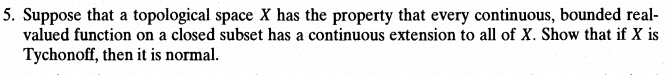
\includegraphics[width=1\textwidth]{12-5.png}
\end{figure}
\end{question}
\begin{solution}
Assume that $X$ is Tychonoff, and let $A$ and $B$ be non-empty disjoint closed subsets of 
$X$. Therefore, $U_A$ is a neighborhood of $A$ and $U_B$ is a neigborhood of $B$, such that
$A \cap B = \emptyset$. Hence, $X$ is normal.

\end{solution}

\bigskip

\begin{question}[2. Royden 12-6]
\hfill
\begin{figure}[h!]
  \centering
    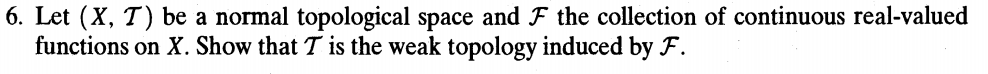
\includegraphics[width=1\textwidth]{12-6}
\end{figure}
\end{question}
\begin{solution}
Consider
\eQb
\mathscr{S} &=& \{ f^{-1}(O) \> | \> f \text{ is continuous, and } O
\text{ is open in} \mathbb{R} \}.
\eQe

\end{solution}

\bigskip

\begin{question}[3. Royden 12-27]
\hfill
\begin{figure}[h!]
  \centering
    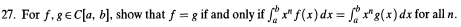
\includegraphics[width=1\textwidth]{12-37}
\end{figure}
\end{question}
\begin{solution}
Consider
\eQb
\mathscr{S} &=& \{ f^{-1}(O) \> | \> f \text{ is continuous, and } O
\text{ is open in} \mathbb{R} \}.
\eQe

\end{solution}

\newpage

\begin{question}[4. Royden 12-35]
\hfill
\begin{figure}[h!]
  \centering
    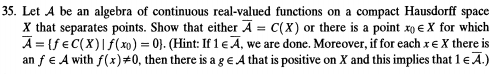
\includegraphics[width=1\textwidth]{12-35}
\end{figure}
\end{question}
\begin{solution}
Consider
\eQb
\mathscr{S} &=& \{ f^{-1}(O) \> | \> f \text{ is continuous, and } O
\text{ is open in} \mathbb{R} \}.
\eQe

\end{solution}

\bigskip

\begin{question}[5. Royden 13-8]
\hfill
\begin{figure}[h!]
  \centering
    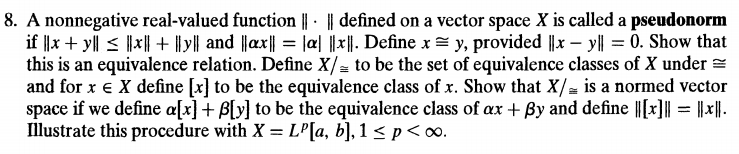
\includegraphics[width=1\textwidth]{13-8}
\end{figure}
\end{question}
\begin{solution}
We show that the relation is reflexive, symmetric, and transitive.

\smallskip

Let $x \in X$. It follows that
\eQb
\lVert x - x \rVert = \lVert \theta \rVert,
\eQe
where $\theta$ is the identity element of the linear space $X$. By definition of linear space,
we have $\alpha \cdot \theta = \theta$ for all $\alpha$. Hence, for some $\alpha > 1$, we have 
\eQb
\lVert \theta \rVert &=& \lVert \alpha \cdot \theta \rVert \\
&=& | \alpha | \lVert \theta \rVert. \\
\eQe
As $|a| > 0$, we have  $|\theta | = 0$. Consequently, $\lVert x - x \rVert = 0$. It follows that
for all $x \in X$, $x \equiv x$. The relation is reflexive. 

\smallskip

Let $x,y \in X$ and $x \equiv y$. Observe that
\eQb
\lVert x - y \rVert &=& \lVert -1\cdot (y - x) \rVert \\
&=& |-1|\lVert y - x \rVert \\
&=& \lVert y - x \rVert. \\
\eQe
As $x \equiv y$, which gives $\lVert x - y \rVert = 0$, it follows that
$\lVert y - x \rVert = 0$ and $y \equiv x$. Hence, the relation is symmetric. 

\smallskip

Let $x,y,z \in X$ and $x \equiv y$ and $y \equiv z$. By triangle inequality, it follows that
\eQb
\lVert y - z \rVert &=& \lVert (x-y) + (y-z) \rVert \\
&\leq& \lVert x -y \rVert + \lVert y - z \rVert = 0 + 0 = 0.
\eQe
Hence, $\lVert y - z\rVert = 0$, and it follows that $x \equiv z$. 
Hence, the relation is symmetric. 

\smallskip 

We show that $X\/_{\equiv}$ is a normed vector space. Firstly, we check that the defined norm
is well defined. Let $x,y \in X$, such that $x \equiv y$. It follows that $\lVert x - y \rVert = 0$.
Hence, $\lVert x \rVert = \lVert y \rVert$, and it follows that $\lVert [x] \rVert = \lVert [y] \rVert$.
The norm is well-defined. 



\end{solution}

\bigskip

\begin{question}[6. Royden 13-33]
\hfill
\begin{figure}[h!]
  \centering
    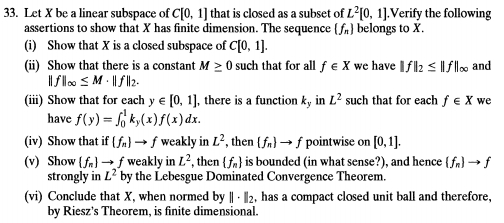
\includegraphics[width=1\textwidth]{13-33}
\end{figure}
\end{question}
\begin{solution}
Consider
\eQb
\mathscr{S} &=& \{ f^{-1}(O) \> | \> f \text{ is continuous, and } O
\text{ is open in} \mathbb{R} \}.
\eQe

\end{solution}

\end{document}
